\documentclass[11pt,a4paper]{ctexart}

\usepackage[margin=2.6cm]{geometry}
\usepackage{amsmath,amssymb,amsthm}
\usepackage{graphicx}
\usepackage{booktabs}
\usepackage{hyperref}
\usepackage{xcolor}
\usepackage{listings}
\usepackage{caption}

\graphicspath{{figures/}}
\hypersetup{colorlinks=true, linkcolor=blue!50!black, urlcolor=blue!60!black}
\lstset{
  basicstyle=\ttfamily\small,
  breaklines=true,
  frame=single,
  columns=fullflexible,
  backgroundcolor=\color{gray!7}
}

\newtheorem{definition}{定义}[section]
\newtheorem{theorem}{定理}[section]
\newtheorem{lemma}{引理}[section]
\newtheorem{proposition}{命题}[section]
\newtheorem{example}{例}[section]

\title{第 14 章 \quad Consistency and asymptotic normality / 一致性与渐近正态性}
\author{基于 \textit{A Course in Time Series Analysis} 的中文讲义与 Python 实践}
\date{}

\begin{document}
\maketitle

\section*{本章学习目标}

本章按照原文 \textit{Consistency and asymptotic normality of estimators} 的小节顺序整理，保留主要定义、定理、模型公式和练习方向，并将原文中的 R 实践思路改写为 Python 工程实践。

完成本章后，应能够：
\begin{itemize}
  \item 区分几乎必然收敛、依概率收敛和分布收敛；
  \item 定义估计量的一致性和渐近正态性；
  \item 掌握 argmax/argmin 一致性定理；
  \item 理解随机等连续和随机 Ascoli 引理；
  \item 应用于 Hannan-Rissanen 和高斯 MLE。
\end{itemize}

\section{收敛模式}

\begin{definition}[收敛，原文 Definition 14.1.1]
若 \(X_n\to X\) 几乎处处，记 \(X_n\xrightarrow{a.s.}X\)；若对任意 \(\epsilon>0\)，
\[
  P(|X_n-X|>\epsilon)\to0,
\]
记 \(X_n\xrightarrow{p}X\)；若分布函数收敛，记 \(X_n\Rightarrow X\)。
\end{definition}

\begin{definition}[有界性，原文 Definition 14.1.2]
\(X_n=O_p(1)\) 表示随机变量序列依概率有界，\(X_n=o_p(1)\) 表示依概率收敛到 0。
\end{definition}

\section{抽样性质与一致性}

\begin{definition}[一致估计，原文 Definition 14.2.1]
若估计量 \(\hat a_n\) 满足
\[
  \hat a_n\xrightarrow{a.s.}a_0
\]
或 \(\hat a_n\xrightarrow{p}a_0\)，则分别称为几乎必然一致或依概率一致。
\end{definition}

\section{估计量的几乎必然收敛}

\begin{definition}[一致收敛，原文 Definition 14.3.1]
若
\[
  \sup_{a\in\Theta}|L_n(a)-L(a)|\xrightarrow{a.s.}0,
\]
称 \(L_n\) 几乎必然一致收敛到 \(L\)。
\end{definition}

\begin{theorem}[Argmax 一致性，原文 Theorem 14.3.1]
若 \(\hat a_n=\arg\max L_n(a)\)，\(a_0=\arg\max L(a)\)，且 \(L_n\) 一致收敛到 \(L\)、\(L\) 的最大点唯一，则 \(\hat a_n\to a_0\)。
\end{theorem}

\section{随机等连续与玩具例子}

\begin{definition}[随机等连续，原文 Definition 14.3.2]
随机函数族在参数空间上若小距离参数点的函数值差可一致控制，则称随机等连续。
\end{definition}

\begin{theorem}[随机 Ascoli 引理，原文 Theorem 14.3.2]
若参数空间紧、随机函数点态收敛且随机等连续，则可推出一致收敛。
\end{theorem}

原文用 AR(1) 估计的玩具例子说明如何把样本目标函数写成极限函数加误差项，并证明
\[
  \hat\phi\xrightarrow{a.s.}\phi.
\]

\section{渐近正态性}

若目标函数 \(L_n(\theta)\) 在真值附近可二阶展开，则一阶条件给出
\[
  0=L_n'(\hat\theta)
  =L_n'(\theta_0)+L_n''(\theta_0)(\hat\theta-\theta_0)+R_n.
\]
若
\[
  \sqrt n L_n'(\theta_0)\Rightarrow N(0,V),
  \qquad
  L_n''(\theta_0)\xrightarrow{p}H,
\]
则
\[
  \sqrt n(\hat\theta-\theta_0)\Rightarrow N(0,H^{-1}VH^{-1}).
\]

\section{Hannan-Rissanen 与 GMLE 渐近性质}

原文后半部分把上述工具用于 Hannan-Rissanen 估计和 ARMA 高斯最大似然。核心任务是证明初步 AR 近似误差足够小、目标函数一致收敛，并用 Taylor 展开得到渐近正态性。

\section{原文定理链补充}

\subsection{随机 Ascoli 证明}
\begin{lemma}[原文 Lemma 14.3.1]
若随机函数列点态收敛且随机等连续，则可推出一致收敛。这是随机 Ascoli 定理证明中的关键步骤。
\end{lemma}

\subsection{AR(1) 玩具例子}
\begin{theorem}[原文 Theorem 14.4.1]
对 AR(1) 估计量 \(\hat\phi\)，在稳定和矩条件下有
\[
  \hat\phi\xrightarrow{a.s.}\phi.
\]
该例展示如何用目标函数极值和遍历定理证明强相合。
\end{theorem}

\subsection{Hannan-Rissanen 渐近性质}
\begin{theorem}[原文 Theorem 14.7.1--14.7.2]
在 ARMA 根条件和高阶 AR 近似阶数合适时，Hannan-Rissanen 初步估计满足所需收敛率，并可进入后续渐近正态证明。
\end{theorem}

\begin{theorem}[原文 Theorem 14.7.3]
ARMA 过程的依赖衰减和矩界给出估计误差的几乎必然控制；附录 B 详细证明该技术结果。
\end{theorem}

\subsection{GMLE 渐近性质}
\begin{proposition}[原文 Proposition 14.8.1--14.8.2]
精确预测、截断预测和近似预测对应的高斯似然在大样本下差异可控，因此它们给出的估计量具有相同一阶渐近性质。
\end{proposition}

\begin{theorem}[原文 Theorem 14.8.1--14.8.2]
在 Assumption 14.8.1 等正则条件下，ARMA 高斯最大似然估计量相合，并且精确似然与近似似然估计量渐近等价。
\end{theorem}

\section{Python 工程实践}

在本章目录下运行：
\begin{lstlisting}[language=bash]
python scripts/ch14_generate_figures.py
\end{lstlisting}

脚本会把图像写入本章 \texttt{figures/} 目录。当前图像用于配合本章核心概念的仿真说明；若后续补齐原始数据文件，可把模拟数据替换为原文真实数据案例。

\begin{figure}[htbp]
  \centering
  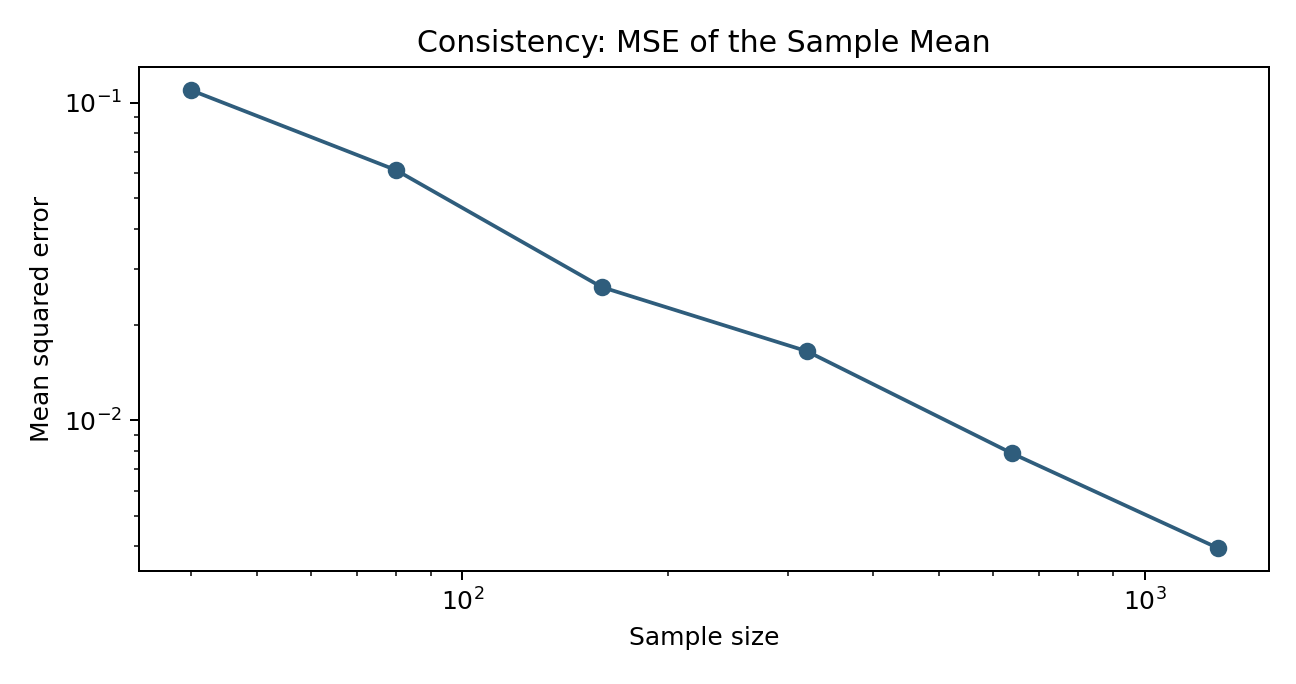
\includegraphics[width=0.86\textwidth]{ch14_fig01_consistency_mse.png}
  \caption{一致性示意：样本量增大时样本均值的均方误差下降。}
\end{figure}

\begin{figure}[htbp]
  \centering
  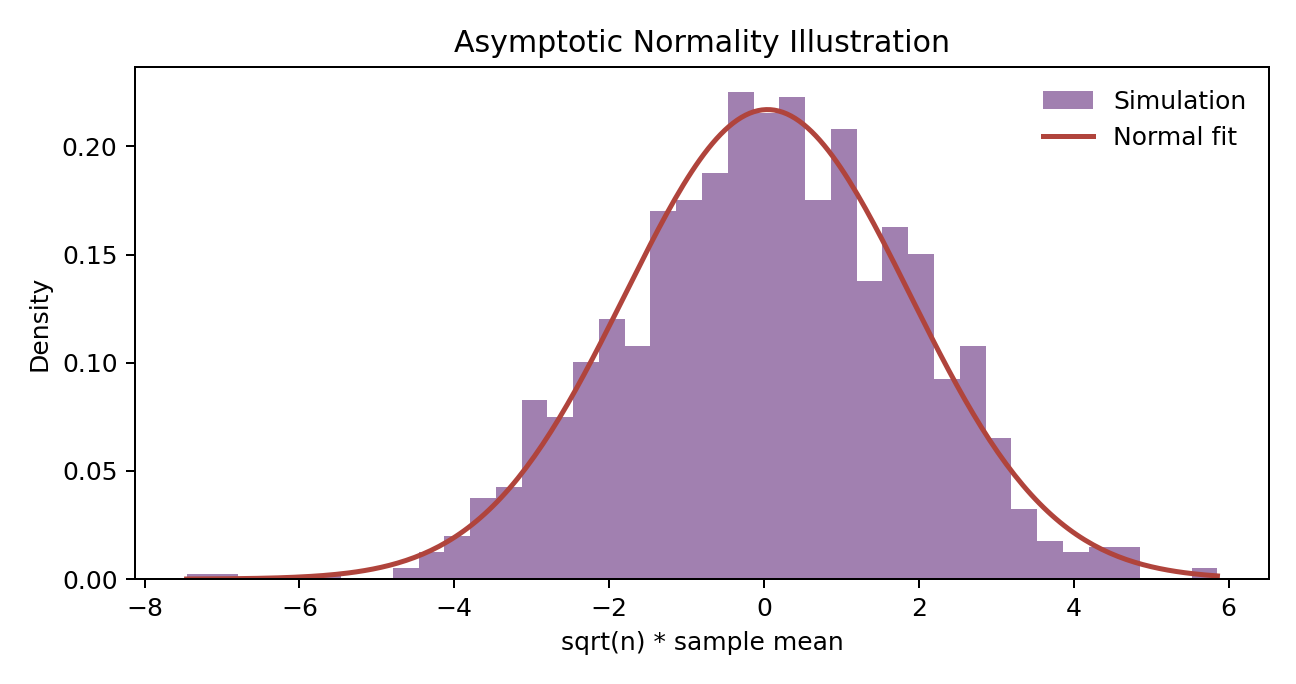
\includegraphics[width=0.86\textwidth]{ch14_fig02_asymptotic_normality.png}
  \caption{渐近正态性示意：标准化估计误差逐渐接近正态分布。}
\end{figure}

\section{练习提要}

原文练习主要围绕下列方向展开：
\begin{itemize}
  \item 判断不同收敛模式之间的关系；
  \item 验证一个目标函数的一致收敛；
  \item 用 AR(1) 估计推导一致性；
  \item 对 M 估计量做 Taylor 展开得到渐近正态。
\end{itemize}

\section*{本章小结}

第 14 章是全书理论证明工具箱。一致性来自目标函数的统一收敛和唯一极值，渐近正态性来自一阶条件、Taylor 展开和中心极限定理；这些工具支撑前面估计方法的抽样性质。

\end{document}
